\section{Hardware Architecture}

\begin{frame}
\frametitle{Hardware Architecture}
The hardware used in an autonomous vehicle project evolves with the different
stages of development.

\begin{itemize}
    \item \textbf{Research}: Off-the-shelf hardware (x86 PCs, network switches, etc.) are used
        in early stages of development in order to focus on the functional
        software.
    \item \textbf{Pre-development}: Evaluation boards from chip vendors, or ruggedized version from
        third parties, are often used in pre-development stages to begin
        the work of optimizing the software for an embedded environment.
    \item \textbf{Production}: Hardware is produced in cooperation with a Tier 1
        supplier (e.g. Continental, ZF, Bosch, etc.), where several samples
        (A-sample to D-sample) are produced before the final version is made
        for start of production (SOP).
\end{itemize}
\end{frame}

\begin{frame}
\frametitle{Hardware Architecture}
\framesubtitle{Early prototyping}
Example of an early prototype with off-the-shelf hardware, but also prototype
hardware from automotive vendors (VIGEM, Elektrobit seen here).
\begin{center}
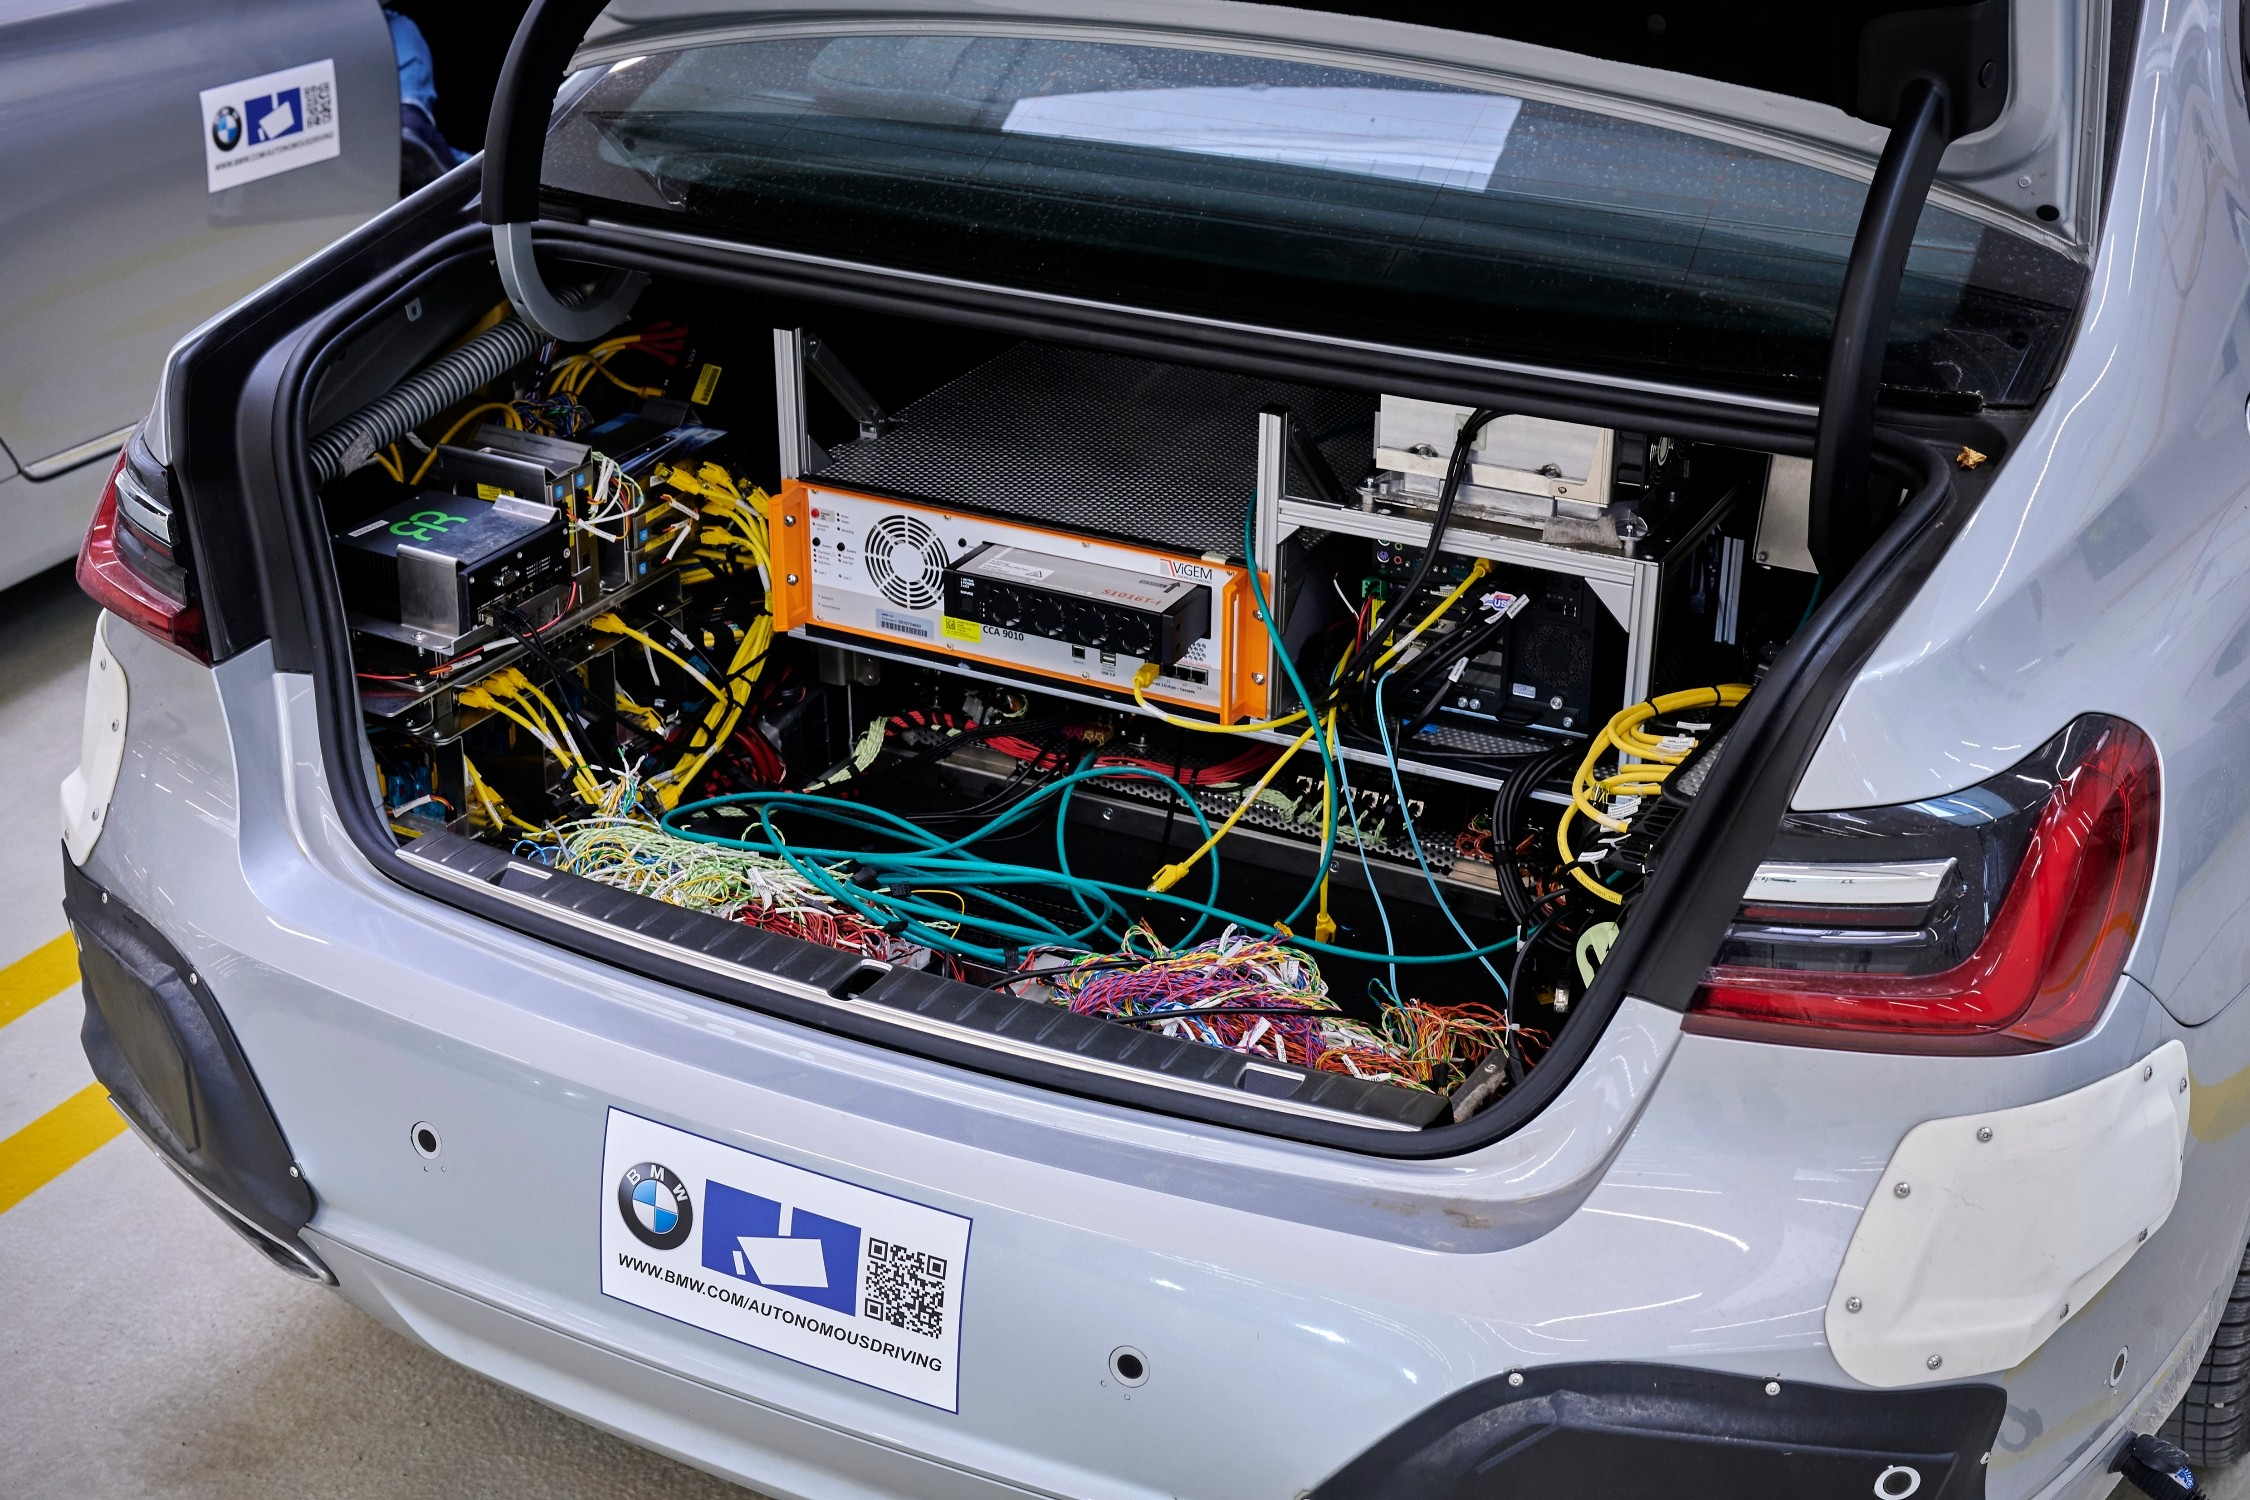
\includegraphics[width=0.5\textwidth]{images/bmw_vehicle_trunk.jpg}\\
\footnotesize Source: BMW\footnotemark[1]
\end{center}
\footnotetext[1]{\tiny{\url{https://www.press.bmwgroup.com/global/article/detail/T0320230EN/nextgen-2020}}}
\end{frame}

\begin{frame}
\frametitle{Hardware Architecture}
\framesubtitle{First embedded hardware}
Developer kits from chip vendors serve as a good platform for doing an initial
integration of a system to an embedded environment and optimizing the
application.
\begin{center}
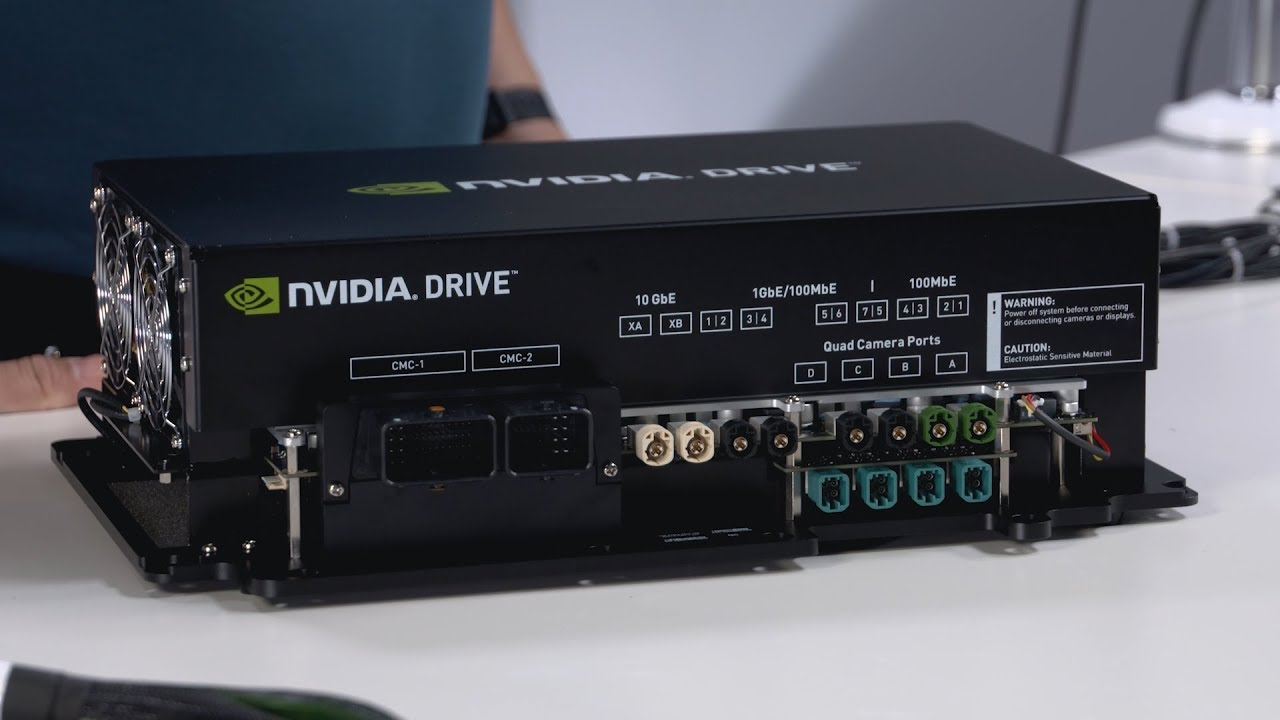
\includegraphics[width=0.6\textwidth]{images/nvidia_drive_agx.jpg}\\
\footnotesize Source: NVIDIA\footnotemark[1]
\end{center}    
\footnotetext[1]{\tiny{\url{https://developer.nvidia.com/drive/drive-agx}}}
\end{frame}

\begin{frame}
\frametitle{Hardware Architecture}
\framesubtitle{Production hardware}
Tier 1 suppliers develop rugged and automotive grade ECUs for mass production,
often customized for an OEM's specific requirements.\\
\vspace{0.2cm}
\begin{columns}[]
    \begin{column}{0.5\textwidth}
        \centering
        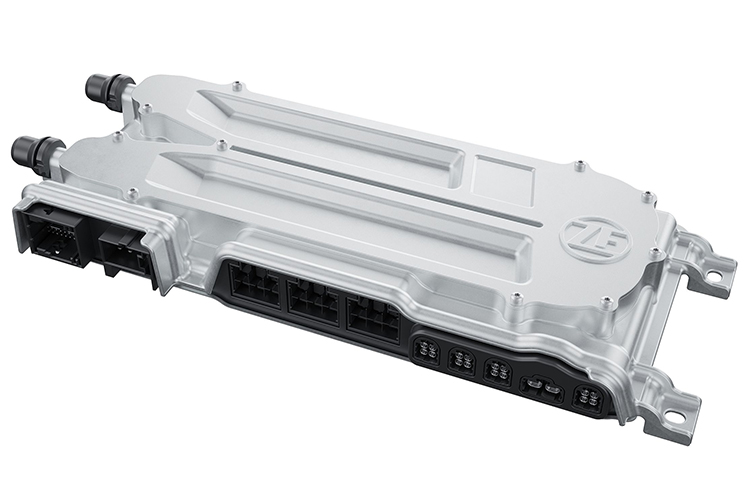
\includegraphics[width=0.7\textwidth]{images/zf_proai_s500l.jpg}\\
        \footnotesize ZF ProAI S500L\footnotemark[1]
    \end{column}
    \begin{column}{0.5\textwidth}
        \centering
        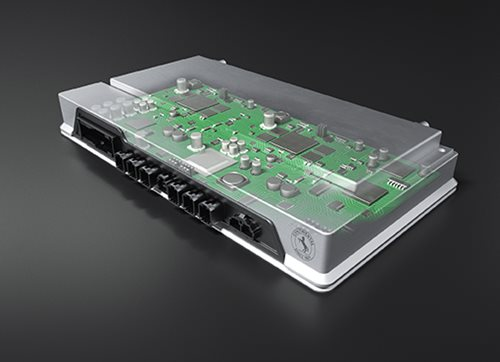
\includegraphics[width=0.7\textwidth]{images/continental_ecu.jpg}\\
        \footnotesize Continental ADAS/AD ECU\footnotemark[2]
    \end{column}
\end{columns}
\footnotetext[1]{\tiny{\url{https://www.zf.com/products/en/cars/stories/proai.html}}}
\footnotetext[2]{\tiny{\url{https://www.continental-automotive.com/en-gl/Passenger-Cars/Autonomous-Mobility/Enablers/Control-Units/Assisted-Automated-Driving-Control-Unit}}}
\end{frame}

\begin{frame}
\frametitle{Hardware Architecture}
\framesubtitle{Designing for safety and performance}
A single, modern ECU designed to be a central domain controller for a vehicle
may contain several different processing units to achieve the overall goals
of safety and performance.

\begin{itemize}
    \item CPUs at the core of the computing, mostly ARM-based architectures
    \item Hardware accelerators for specific tasks: GPUs, DSPs, NPUs, etc.
    \item Customized computing: ASICs, FPGAs
    \item Safety-critical microcontrollers
    \item SPI, Ethernet, PCI Express, hardware shared memory, etc. for
        communication between computing cores
    \item SOCs may combines several types of computing cores onto a single chip
\end{itemize}
\end{frame}

\begin{frame}
\frametitle{Hardware Architecture}
\framesubtitle{Current 4th-Gen architectures and future 5th-Gen architectures}
\small{Automotive vehicle-wide ECU architectures are evolving and undergoing
drastic changes. Hardware complexity is being reduced by integrating fewer,
but more powerful, ECUs.}
%\vspace{0.1cm}
\begin{columns}[]
    \begin{column}{0.6\textwidth}
        \centering
        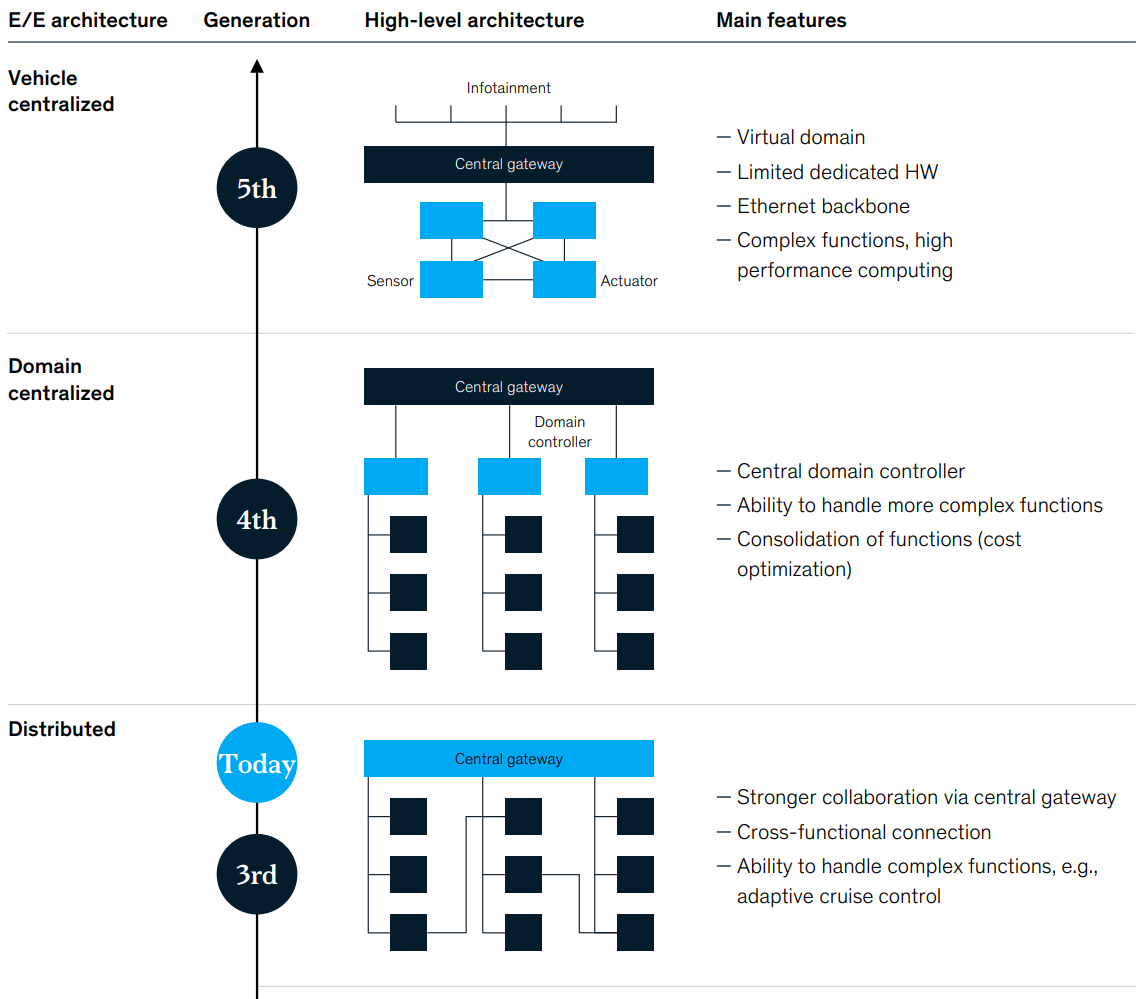
\includegraphics[width=0.65\textwidth]{images/mckinsey_vehicle_architecture_generations.png}\\
        \tiny Evolution from 3rd Gen to 5th Gen architectures \cite{McKinseyReport}
    \end{column}
    \begin{column}{0.4\textwidth}
        \centering
        \includesvg[svgextension=svgz,height=0.55\textheight]{images/mckinsey_hw_architecture_5th_gen_zonal.svgz}\\
        \tiny{5th Gen Zonal Architecture\footnotemark[1]}
    \end{column}
\end{columns}
\footnotetext[1]{\tiny{\url{https://www.mckinsey.com/industries/automotive-and-assembly/our-insights/rewiring-car-electronics-and-software-architecture-for-the-roaring-2020s}}}
\end{frame}
